\section{The interpreter}

The interpreter of \asl\ has been designed using ANTLRv3 and Java.
The interpreter is installed by executing a \texttt{``make''} command
in the root directory of the \asl\ distribution. The user might need to
redefine the variables \texttt{ANTLR\_ROOT} and \texttt{JAVA\_LIBS}
to specify the location of ANTLR and Java libraries.

The interpreter is invoked by executing the command \texttt{Asl <file>}.
The interpreter can also be invoked with some options that can be
listed by running \texttt{Asl -help}:

\begin{verbatim}
$ Asl -help
usage: Asl [options] file
 -ast <file>     write the AST
 -dot            dump the AST in dot format
 -help           print this message
 -noexec         do not execute the program
 -trace <file>   write a trace of function calls during the execution of
                 the program
\end{verbatim}

The option \texttt{-ast} generates a textual representation of the Abstract
Syntax Tree (AST) in dot format. If the \texttt{-dot} option is used, the
representation is in dot format, that can be later transformed into
some graphical format using \texttt{dot}, e.g.:

\begin{verbatim}
$ Asl fact.asl -ast fact.dot -dot -noexec
$ dot -Tpdf -o fact.pdf fact.dot
\end{verbatim}

The option \texttt{-noexec} must be used when the user does not want
to execute the program. It is useful when only a visualization of the AST is
required.

Figure~\ref{fig:ast} depicts the AST of the first example used in this
document.

\begin{figure}
 \centering
 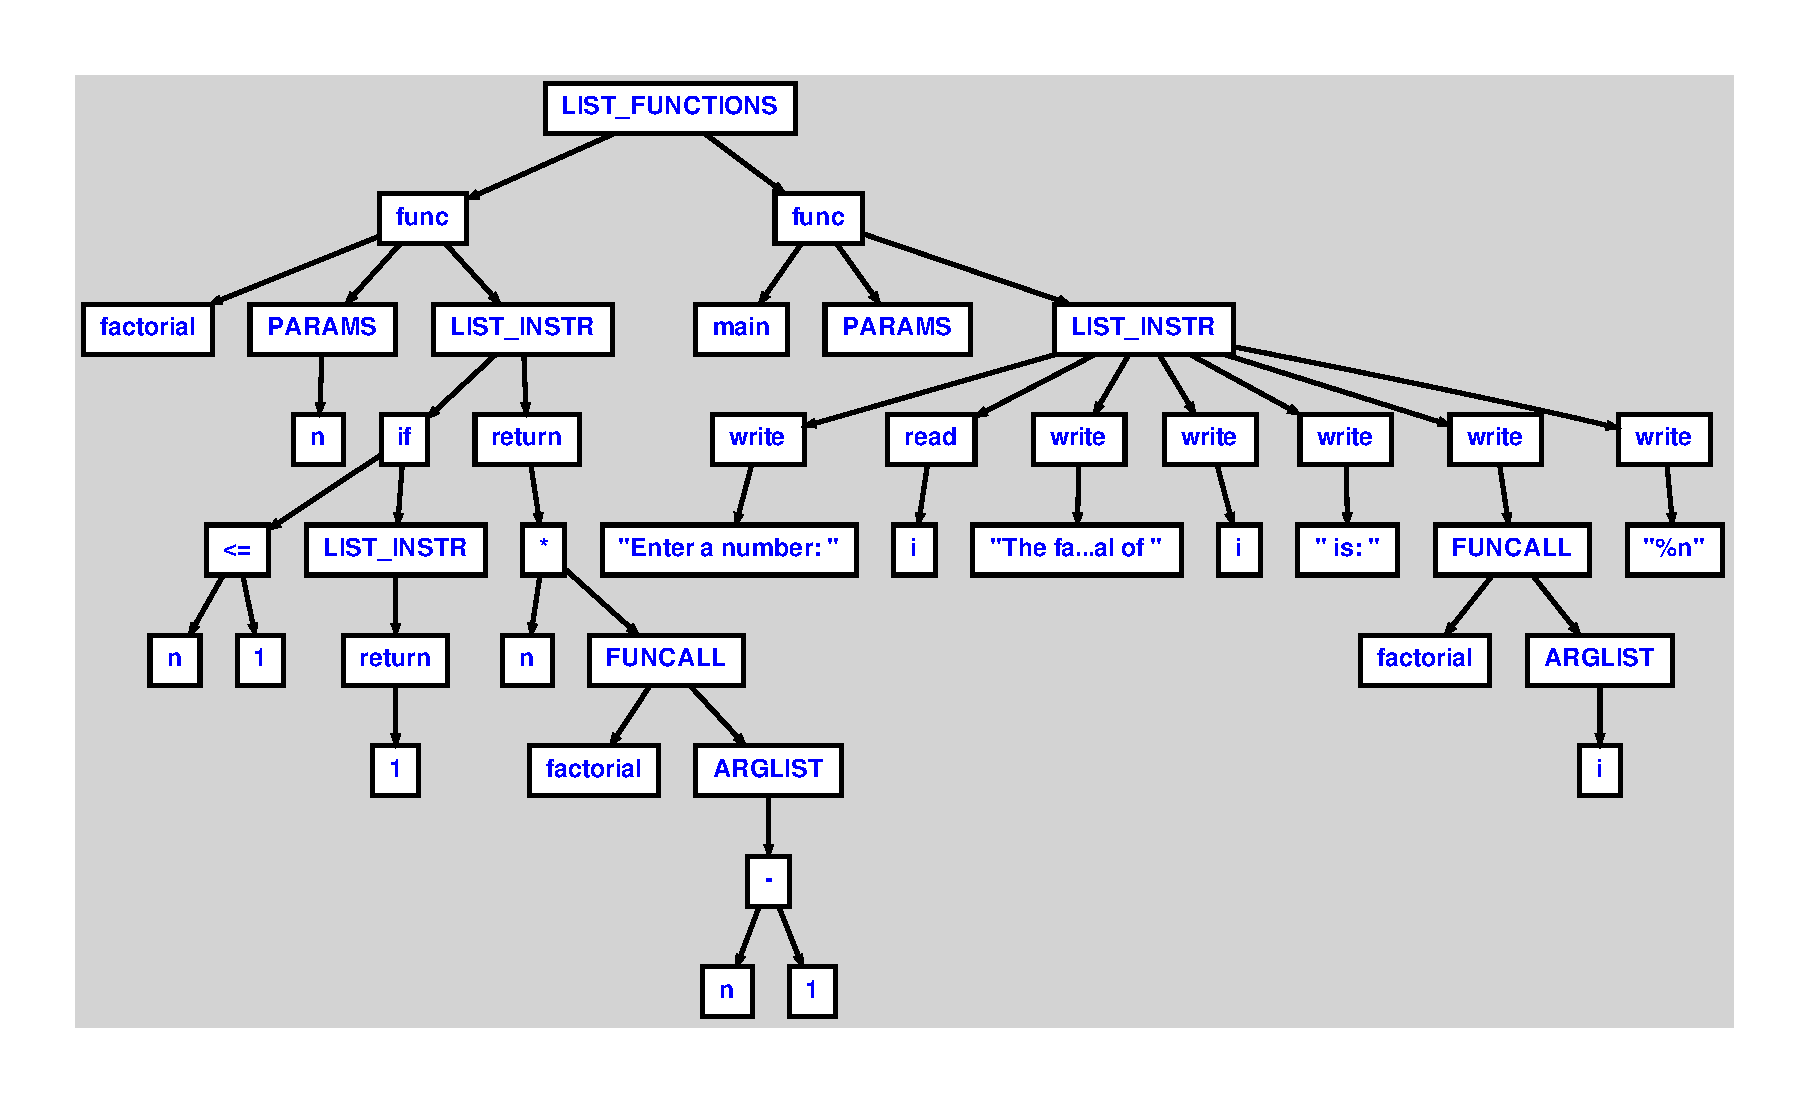
\includegraphics[width=\linewidth]{./fact.pdf}
 % fact.pdf: 867x528 pixel, 72dpi, 30.59x18.63 cm, bb=0 0 867 528
 \caption{AST of the factorial example.}
 \label{fig:ast}
\end{figure}

The option \texttt{-noexec} must be used when the user does not want
to execute the program. It is useful when only a visualization of the AST is
required.

The option \texttt{-trace} can be used for debugging. For example, let us
consider the following program that generates the moves for the problem of
Hanoi towers.

\begin{verbatim}
 1:    func main()
 2:      write "Number of disks: "; read n;
 3:      nmoves = 0;
 4:      hanoi(n, 1, 2, 3, nmoves);
 5:      write "Total number of moves: "; write nmoves; write "%n";
 6:    endfunc
 7:
 8:    func hanoi(n, from, aux, to, &mov)
 9:      if n > 0 then
10:        hanoi(n-1, from, aux, to, mov);
11:        write "Move from "; write from;
12:        write " to "; write to; write "%n";
13:        mov = mov + 1;
14:        hanoi(n-1, aux, to, from, mov);
15:      endif
16:    endfunc
\end{verbatim}

In this example, the parameter \texttt{mov} is passed by reference and
accumulates the number of moves. The rods are represented by the numbers 1, 2
and 3.

The execution the program with 3 disks would look as follows:

\begin{verbatim}
  $ Asl hanoi.asl -trace hanoi.trace 
  Number of disks: 3
  Move from 1 to 3
  Move from 1 to 3
  Move from 2 to 1
  Move from 1 to 3
  Move from 2 to 1
  Move from 2 to 1
  Move from 3 to 2
  Total number of moves: 7
\end{verbatim}

The file \texttt{hanoi.trace} reports the trace of function calls
and returns with the values of the parameters and returned data.
It also reports the value of the variables passed by reference
at the return of each function. The contents of the file is the following:

\begin{verbatim}
main() <entry point>
|   hanoi(n=3, from=1, aux=2, to=3, &mov=0) <line 4>
|   |   hanoi(n=2, from=1, aux=2, to=3, &mov=0) <line 10>
|   |   |   hanoi(n=1, from=1, aux=2, to=3, &mov=0) <line 10>
|   |   |   |   hanoi(n=0, from=1, aux=2, to=3, &mov=0) <line 10>
|   |   |   |   return, &mov=0 <line 9>
|   |   |   |   hanoi(n=0, from=2, aux=3, to=1, &mov=1) <line 14>
|   |   |   |   return, &mov=1 <line 9>
|   |   |   return, &mov=1 <line 9>
|   |   |   hanoi(n=1, from=2, aux=3, to=1, &mov=2) <line 14>
|   |   |   |   hanoi(n=0, from=2, aux=3, to=1, &mov=2) <line 10>
|   |   |   |   return, &mov=2 <line 9>
|   |   |   |   hanoi(n=0, from=3, aux=1, to=2, &mov=3) <line 14>
|   |   |   |   return, &mov=3 <line 9>
|   |   |   return, &mov=3 <line 9>
|   |   return, &mov=3 <line 9>
|   |   hanoi(n=2, from=2, aux=3, to=1, &mov=4) <line 14>
|   |   |   hanoi(n=1, from=2, aux=3, to=1, &mov=4) <line 10>
|   |   |   |   hanoi(n=0, from=2, aux=3, to=1, &mov=4) <line 10>
|   |   |   |   return, &mov=4 <line 9>
|   |   |   |   hanoi(n=0, from=3, aux=1, to=2, &mov=5) <line 14>
|   |   |   |   return, &mov=5 <line 9>
|   |   |   return, &mov=5 <line 9>
|   |   |   hanoi(n=1, from=3, aux=1, to=2, &mov=6) <line 14>
|   |   |   |   hanoi(n=0, from=3, aux=1, to=2, &mov=6) <line 10>
|   |   |   |   return, &mov=6 <line 9>
|   |   |   |   hanoi(n=0, from=1, aux=2, to=3, &mov=7) <line 14>
|   |   |   |   return, &mov=7 <line 9>
|   |   |   return, &mov=7 <line 9>
|   |   return, &mov=7 <line 9>
|   return, &mov=7 <line 9>
return <line 5>
\end{verbatim}

\subsection{Organization of the interpreter}

\begin{figure}
\Tree [.\fbox{\textbf{src}} 
[.\fbox{\textbf{Asl}} Asl.java ]
[.\fbox{\textbf{parser}} 
  Asl.g\\\emph{AslLexer.java}\\\emph{AslParser.java}\\\emph{Asl.tokens} ]
[.\fbox{\textbf{interp}} 
  Interp.java\\Data.java\\Memory.java\\AslTree.java\\AslTreeAdaptor.java ]
]
\caption{Structure of the \texttt{src} directory containing the source files
of the interpreter.}
\label{fig:src}
\end{figure}

The source files of the interpreter are organized in three packages
(see Fig.~\ref{fig:src}):
\begin{description}
 \item [Asl:] contains the class \texttt{Asl} with the entry point
(\texttt{main}) of the program. It calls the \emph{parser} and
\emph{interpreter}.
\item [parser:] contains the grammar and creator of the AST.
In the original distribution, this directory only contains the file
\texttt{Asl.g}. The other files (italics in Fig.~\ref{fig:src}) are
created by ANTLR.
\item [interp:] contains the interpreter of the AST organized in different
files:
\begin{itemize}
 \item \emph{Interp.java}. It contains the core of the interpreter,
traversing the AST and executing the instructions.
\item \emph{Data.java}. It contains the class to represent data values
(integer and Boolean) and execute operations on them.
\item \emph{Memory.java}. It implements the memory of the interpreter with a
stack of activation records that contain pairs of strings (variable names)
and data (values).
\item \emph{AslTree.java}. It contains a subclass of the AST that extends the
information included in every AST node.
\item \emph{AslTreeAdaptor.java}. It contains a subclass required by ANTLR to
have access to the extended AST.
\end{itemize}
\end{description}

\subsubsection{Interp.java}

It has two public functions:
\begin{itemize}
 \item \texttt{Interp(AslTree T)}. This is the constructor of the
interpreter. It prepares the AST for the interpretation. It also creates a
table that maps function names into AST nodes (the roots of the functions).
The parameter \texttt{T} is the root of the AST.

\item \texttt{void Run()}. It runs the program by interpreting the AST.
\end{itemize}

Inside this file, there are some essential functions that constitute the
core of the interpreter. They execute function calls and instructions and
evaluate expressions.

\begin{itemize}
 \item \texttt{Data executeFunction(String funcname, AslTree args)}. This
function executes a function with a given name in which \texttt{args}
contains the AST of the list of arguments passed by the caller. The function
also implements the parameter passing mechanism.

\item \texttt{Data executeInstruction(AslTree t)}. This function executes
an individual instruction. In case the instruction returns some data (i.e. a
\texttt{return} instruction or some block of instructions that contains a
\texttt{return}), this function returns the data. Otherwise, a \texttt{null}
is returned.

\item \texttt{Data evaluateExpression(AslTree t)}. This function returns the
value produced by the evaluation of the expression represented by an AST.
\end{itemize}

During the execution of a program, the interpreter performs various semantic
and execution checks (access to undefined variables, operations with
incompatible types, division by zero, etc.) that may raise runtime exceptions.
The interpreter also keeps track of the line number of the source program for
an appropriate debugging when an exception is produced.

\subsubsection{Data.java}

This class represents a data item stored in memory. It provides methods to
retrieve the type and value of the data and perform arithmetic, logical and
relational operations. It also contains methods for semantic and runtime
checks.

\subsubsection{Memory.java}

This class represents the memory of the virtual machine that interprets
the program. \asl\ does not have global variables, thus all the visible
variables are local. Data can only be shared through the pass of parameters
or return of results. Parameters can be pass by value or reference.

Figure~\ref{fig:ar} depicts the structure of the memory. Each function has an
associated \emph{activation record} (AR) that stores all the variables in the
scope. When a new function is called, a new AR is created. The AR is
destroyed when the function terminates. Therefore, the memory is organized
as a stack of ARs.

\begin{figure}
\begin{center}
\begin{tabular}{|c|c|}
\multicolumn{2}{c}{\textbf{AR(\texttt{main})}} \\
\hline
\textbf{name} & \textbf{value} \\ \hline 
\texttt{n} & 7 \\
\texttt{done} & \emph{false} \\
 & \\
\vdots & \vdots \\
\hline
\end{tabular}
$\longrightarrow$
\begin{tabular}{|c|c|}
\multicolumn{2}{c}{\textbf{AR(\texttt{f})}} \\
\hline
\textbf{name} & \textbf{value} \\ \hline 
\texttt{param1} & 1 \\
\texttt{param2} & \texttt{@main.n} \\
\texttt{found} & \emph{true} \\
\vdots & \vdots \\
\hline
\end{tabular}
$\longrightarrow$
\begin{tabular}{|c|c|}
\multicolumn{2}{c}{\textbf{AR(\texttt{g})}} \\
\hline
\textbf{name} & \textbf{value} \\
\hline 
\texttt{size} & 1000 \\
\texttt{flag} & \emph{false} \\
\texttt{sum} & 23 \\
\vdots & \vdots \\
\hline
\end{tabular}
\end{center}
\caption{Dynamic organization of the memory as a stack of activation
records(AR).}
\label{fig:ar}
\end{figure}

Each AR contains a set of entries with pairs
$\langle\texttt{name},\textit{value}\rangle$. When an entry represents a
parameter passed by reference, the \emph{value} is a reference to another
entry in another AR. The entries in the ARs are created at runtime each time
a new variable is defined.

\subsection{AslTree.java and AslTreeAdaptor.java}

These two files contain two classes that are required to extend the
information of the AST nodes. ANTLR allows this extension by creating
a subclass of the default class to represent AST nodes (\texttt{CommonTree}).

The extension implemented in \asl\ is very simple and allows to store the
integer and Boolean literals as Java \texttt{int}'s. This avoids the burden
to parse a text representation each time the literal needs to be read.

The class \texttt{AslTree} can be further extended for other purposes.
